\documentclass[twoside]{book}

% Packages required by doxygen
\usepackage{fixltx2e}
\usepackage{calc}
\usepackage{doxygen}
\usepackage[export]{adjustbox} % also loads graphicx
\usepackage{graphicx}
\usepackage[utf8]{inputenc}
\usepackage{makeidx}
\usepackage{multicol}
\usepackage{multirow}
\PassOptionsToPackage{warn}{textcomp}
\usepackage{textcomp}
\usepackage[nointegrals]{wasysym}
\usepackage[table]{xcolor}

% Font selection
\usepackage[T1]{fontenc}
\usepackage[scaled=.90]{helvet}
\usepackage{courier}
\usepackage{amssymb}
\usepackage{sectsty}
\renewcommand{\familydefault}{\sfdefault}
\allsectionsfont{%
  \fontseries{bc}\selectfont%
  \color{darkgray}%
}
\renewcommand{\DoxyLabelFont}{%
  \fontseries{bc}\selectfont%
  \color{darkgray}%
}
\newcommand{\+}{\discretionary{\mbox{\scriptsize$\hookleftarrow$}}{}{}}

% Page & text layout
\usepackage{geometry}
\geometry{%
  a4paper,%
  top=2.5cm,%
  bottom=2.5cm,%
  left=2.5cm,%
  right=2.5cm%
}
\tolerance=750
\hfuzz=15pt
\hbadness=750
\setlength{\emergencystretch}{15pt}
\setlength{\parindent}{0cm}
\setlength{\parskip}{3ex plus 2ex minus 2ex}
\makeatletter
\renewcommand{\paragraph}{%
  \@startsection{paragraph}{4}{0ex}{-1.0ex}{1.0ex}{%
    \normalfont\normalsize\bfseries\SS@parafont%
  }%
}
\renewcommand{\subparagraph}{%
  \@startsection{subparagraph}{5}{0ex}{-1.0ex}{1.0ex}{%
    \normalfont\normalsize\bfseries\SS@subparafont%
  }%
}
\makeatother

% Headers & footers
\usepackage{fancyhdr}
\pagestyle{fancyplain}
\fancyhead[LE]{\fancyplain{}{\bfseries\thepage}}
\fancyhead[CE]{\fancyplain{}{}}
\fancyhead[RE]{\fancyplain{}{\bfseries\leftmark}}
\fancyhead[LO]{\fancyplain{}{\bfseries\rightmark}}
\fancyhead[CO]{\fancyplain{}{}}
\fancyhead[RO]{\fancyplain{}{\bfseries\thepage}}
\fancyfoot[LE]{\fancyplain{}{}}
\fancyfoot[CE]{\fancyplain{}{}}
\fancyfoot[RE]{\fancyplain{}{\bfseries\scriptsize Generated by Doxygen }}
\fancyfoot[LO]{\fancyplain{}{\bfseries\scriptsize Generated by Doxygen }}
\fancyfoot[CO]{\fancyplain{}{}}
\fancyfoot[RO]{\fancyplain{}{}}
\renewcommand{\footrulewidth}{0.4pt}
\renewcommand{\chaptermark}[1]{%
  \markboth{#1}{}%
}
\renewcommand{\sectionmark}[1]{%
  \markright{\thesection\ #1}%
}

% Indices & bibliography
\usepackage{natbib}
\usepackage[titles]{tocloft}
\setcounter{tocdepth}{3}
\setcounter{secnumdepth}{5}
\makeindex

% Hyperlinks (required, but should be loaded last)
\usepackage{ifpdf}
\ifpdf
  \usepackage[pdftex,pagebackref=true]{hyperref}
\else
  \usepackage[ps2pdf,pagebackref=true]{hyperref}
\fi
\hypersetup{%
  colorlinks=true,%
  linkcolor=blue,%
  citecolor=blue,%
  unicode%
}

% Custom commands
\newcommand{\clearemptydoublepage}{%
  \newpage{\pagestyle{empty}\cleardoublepage}%
}

\usepackage{caption}
\captionsetup{labelsep=space,justification=centering,font={bf},singlelinecheck=off,skip=4pt,position=top}

%===== C O N T E N T S =====

\begin{document}

% Titlepage & ToC
\hypersetup{pageanchor=false,
             bookmarksnumbered=true,
             pdfencoding=unicode
            }
\pagenumbering{alph}
\begin{titlepage}
\vspace*{7cm}
\begin{center}%
{\Large P2P \\[1ex]\large 1 }\\
\vspace*{1cm}
{\large Generated by Doxygen 1.8.13}\\
\end{center}
\end{titlepage}
\clearemptydoublepage
\pagenumbering{roman}
\tableofcontents
\clearemptydoublepage
\pagenumbering{arabic}
\hypersetup{pageanchor=true}

%--- Begin generated contents ---
\chapter{p2p\+\_\+stri}
\label{index}\hypertarget{index}{}This Java project is developped in collaboration with Romain B\+R\+E\+D\+A\+R\+I\+OL \& Léo-\/\+Paul Dewitte.

\doxysection*{Goal}

This application act as a P2P Client to share files.

\doxysection*{Subject}

{\bfseries{But}} \+: le but de ce projet est de créer une application répartie en Java de téléchargement de fichier en mode P2P (peer to peer ou poste à poste). Les étapes suivantes sont conseillées. \doxysubsection*{Étape 1 \+: Téléchargement à la F\+TP}

La première étape doit permettre de télécharger un fichier en intégralité d\textquotesingle{}une machine vers une autre machine de façon similaire aux applications suivant le protocole F\+TP.

Plan de travail \+:


\begin{DoxyItemize}
\item Lire le sujet jusqu\textquotesingle{}au bout et la R\+FC F\+TP (version anglaise, version française)
\item Concevoir l\textquotesingle{}application répartie avec U\+ML
\item Écrire l\textquotesingle{}application serveur et l\textquotesingle{}application cliente.
\end{DoxyItemize}

\doxysubsection*{Étape 2 \+: Téléchargement en parallèle}

Dans la seconde étape, on permet à un client de télécharger le fichier depuis plusieurs serveurs. Le fichier sera découpé en plusieurs blocs de tailles égales (par exemple 4 Ko) qui seront téléchargés depuis plusieurs serveurs. Dans cette étape c\textquotesingle{}est le client qui choisit (par exemple aléatoirement) quel bloc télécharger depuis quel serveur.

Plan de travail \+:


\begin{DoxyItemize}
\item Modifier le serveur pour gérer l\textquotesingle{}envoi de n\textquotesingle{}importe quel bloc d\textquotesingle{}un fichier
\item Modifier le client pour qu\textquotesingle{}il puisse demander le téléchargement de n\textquotesingle{}importe quel bloc et re-\/créer le fichier complet.
\end{DoxyItemize}

\doxysubsection*{Étape 3 \+: Transformation en P2P simple}

Dans cette étape, il n\textquotesingle{}y a plus de clients ni de serveurs ; les applications sont les deux à la fois. Chaque application devra noter de quelle partie du fichier elle dispose. Au démarrage certaines applications auront le fichier complet et les autres aucun bloc. Les applications demanderont aléatoirement chaque bloc manquant à n\textquotesingle{}importe quelle autre application qui renverra soit le bloc soit un message d\textquotesingle{}erreur.

\doxysubsection*{Étape 4 \+: P2P coordonné}

Dans cette étape, on ajoute un serveur dont le rôle est de maintenir la liste des applications gérant le téléchargement d\textquotesingle{}un fichier et quel bloc chaque application possède. Ce serveur coordonnera le téléchargement en précisant à chaque application, à qui se connecter et ce qui y est disponible.

\doxysubsection*{Étape 5 \+: P2P coopératif}

Dans cette étape, on doit s\textquotesingle{}assurer que les applications envoient et reçoivent globalement les même quantités. On essaiera ainsi de désavantager les applications qui ne font que télécharger et n\textquotesingle{}envoient rien.

\doxysubsection*{Options \+:}


\begin{DoxyItemize}
\item Créer une I\+HM (interface homme machine) Graphique pour les applications avec Swing par exemple.
\item Gérer à la fois des communications U\+DP et T\+CP. 
\end{DoxyItemize}
\chapter{Hierarchical Index}
\section{Class Hierarchy}
This inheritance list is sorted roughly, but not completely, alphabetically\+:\begin{DoxyCompactList}
\item \contentsline{section}{terminal\+Client.\+Gestionnaire\+Fichier}{\pageref{classterminalClient_1_1GestionnaireFichier}}{}
\item \contentsline{section}{central\+Server.\+Liste\+Des\+Fichiers\+Complets}{\pageref{classcentralServer_1_1ListeDesFichiersComplets}}{}
\item \contentsline{section}{central\+Server.\+Liste\+Des\+Info\+Utilisateur}{\pageref{classcentralServer_1_1ListeDesInfoUtilisateur}}{}
\item \contentsline{section}{commun.\+Messages}{\pageref{classcommun_1_1Messages}}{}
\item Runnable\begin{DoxyCompactList}
\item \contentsline{section}{gestionnaire\+Requete.\+Gestionnaire\+Requetes}{\pageref{classgestionnaireRequete_1_1GestionnaireRequetes}}{}
\begin{DoxyCompactList}
\item \contentsline{section}{gestionnaire\+Requete.\+Gestionnaire\+Requetes\+Serveur}{\pageref{classgestionnaireRequete_1_1GestionnaireRequetesServeur}}{}
\item \contentsline{section}{gestionnaire\+Requete.\+Gestionnaire\+Requetes\+Serveur\+Central}{\pageref{classgestionnaireRequete_1_1GestionnaireRequetesServeurCentral}}{}
\end{DoxyCompactList}
\item \contentsline{section}{requete.\+Requete}{\pageref{classrequete_1_1Requete}}{}
\begin{DoxyCompactList}
\item \contentsline{section}{gestionnaire\+Requete.\+Gestionnaire\+De\+Telechargement}{\pageref{classgestionnaireRequete_1_1GestionnaireDeTelechargement}}{}
\item \contentsline{section}{requete.\+Requete\+Liste}{\pageref{classrequete_1_1RequeteListe}}{}
\item \contentsline{section}{requete.\+Requete\+Telecharger}{\pageref{classrequete_1_1RequeteTelecharger}}{}
\item \contentsline{section}{requete.\+Requete\+Update\+Infos\+Utilisateur}{\pageref{classrequete_1_1RequeteUpdateInfosUtilisateur}}{}
\end{DoxyCompactList}
\item \contentsline{section}{terminal\+Client.\+Gestionnaire\+Infos\+Utilisateur}{\pageref{classterminalClient_1_1GestionnaireInfosUtilisateur}}{}
\item \contentsline{section}{terminal\+Client.\+Serveur}{\pageref{classterminalClient_1_1Serveur}}{}
\end{DoxyCompactList}
\item \contentsline{section}{central\+Server.\+Serveur\+Central}{\pageref{classcentralServer_1_1ServeurCentral}}{}
\item \contentsline{section}{central\+Server.\+Serveur\+Central\+Main}{\pageref{classcentralServer_1_1ServeurCentralMain}}{}
\item \contentsline{section}{terminal\+Client.\+Terminal\+Main}{\pageref{classterminalClient_1_1TerminalMain}}{}
\item Serializable\begin{DoxyCompactList}
\item \contentsline{section}{commun.\+Info\+Utilisateur}{\pageref{classcommun_1_1InfoUtilisateur}}{}
\item \contentsline{section}{commun.\+Liste\+De\+Blocs}{\pageref{classcommun_1_1ListeDeBlocs}}{}
\end{DoxyCompactList}
\end{DoxyCompactList}

\chapter{Class Index}
\section{Class List}
Here are the classes, structs, unions and interfaces with brief descriptions\+:\begin{DoxyCompactList}
\item\contentsline{section}{\hyperlink{classclient_1_1Client}{client.\+Client} }{\pageref{classclient_1_1Client}}{}
\item\contentsline{section}{\hyperlink{classcommon_1_1Messages}{common.\+Messages} }{\pageref{classcommon_1_1Messages}}{}
\item\contentsline{section}{\hyperlink{classserveur_1_1Serveur}{serveur.\+Serveur} }{\pageref{classserveur_1_1Serveur}}{}
\item\contentsline{section}{\hyperlink{classcommon_1_1Socket}{common.\+Socket} \\*Cette classe permet de gérer les sockets }{\pageref{classcommon_1_1Socket}}{}
\end{DoxyCompactList}

\chapter{Class Documentation}
\hypertarget{classcommon_1_1GestionnaireFichier}{}\section{common.\+Gestionnaire\+Fichier Class Reference}
\label{classcommon_1_1GestionnaireFichier}\index{common.\+Gestionnaire\+Fichier@{common.\+Gestionnaire\+Fichier}}


Cette classe gere le dossier contenant les fichiers partagés ainsi que le dossier de téléchargement.  


\subsection*{Public Member Functions}
\begin{DoxyCompactItemize}
\item 
\hyperlink{classcommon_1_1GestionnaireFichier_af063deb28fa952a2d0c605bc26659b16}{Gestionnaire\+Fichier} (String chemin\+Dossier\+Partages, String chemin\+Dossier\+Telechargements)
\begin{DoxyCompactList}\small\item\em constructeur de \hyperlink{classcommon_1_1GestionnaireFichier}{Gestionnaire\+Fichier} \end{DoxyCompactList}\item 
\mbox{\Hypertarget{classcommon_1_1GestionnaireFichier_a7189336732591523f7490df6a16cae34}\label{classcommon_1_1GestionnaireFichier_a7189336732591523f7490df6a16cae34}} 
String {\bfseries liste\+Fichiers} ()
\item 
File\+Input\+Stream \hyperlink{classcommon_1_1GestionnaireFichier_a55da4571d743ce9ee31a96bd04de9aa4}{rechercher\+Fichier} (String nom\+Fichier)  throws File\+Not\+Found\+Exception 
\begin{DoxyCompactList}\small\item\em cette méthode permet d\textquotesingle{}obtenir le stream du fichier à partir d\textquotesingle{}un nom de fichier. \end{DoxyCompactList}\item 
File\+Output\+Stream \hyperlink{classcommon_1_1GestionnaireFichier_a7aa94ceed1766208e16cd4d3ce8465b7}{creer\+Fichier} (String nom\+Fichier)  throws File\+Not\+Found\+Exception 
\begin{DoxyCompactList}\small\item\em créer un nouveau fichier dans le dossier de téléchargement. \end{DoxyCompactList}\end{DoxyCompactItemize}


\subsection{Detailed Description}
Cette classe gere le dossier contenant les fichiers partagés ainsi que le dossier de téléchargement. 

\subsection{Constructor \& Destructor Documentation}
\mbox{\Hypertarget{classcommon_1_1GestionnaireFichier_af063deb28fa952a2d0c605bc26659b16}\label{classcommon_1_1GestionnaireFichier_af063deb28fa952a2d0c605bc26659b16}} 
\index{common\+::\+Gestionnaire\+Fichier@{common\+::\+Gestionnaire\+Fichier}!Gestionnaire\+Fichier@{Gestionnaire\+Fichier}}
\index{Gestionnaire\+Fichier@{Gestionnaire\+Fichier}!common\+::\+Gestionnaire\+Fichier@{common\+::\+Gestionnaire\+Fichier}}
\subsubsection{\texorpdfstring{Gestionnaire\+Fichier()}{GestionnaireFichier()}}
{\footnotesize\ttfamily common.\+Gestionnaire\+Fichier.\+Gestionnaire\+Fichier (\begin{DoxyParamCaption}\item[{String}]{chemin\+Dossier\+Partages,  }\item[{String}]{chemin\+Dossier\+Telechargements }\end{DoxyParamCaption})\hspace{0.3cm}{\ttfamily [inline]}}



constructeur de \hyperlink{classcommon_1_1GestionnaireFichier}{Gestionnaire\+Fichier} 


\begin{DoxyParams}{Parameters}
{\em chemin\+Dossier\+Partages} & chemin complet vers le dossiers contenant les fichiers partagés. accepte uniquement un chemin Linux car Linux $>$ Windows. \\
\hline
\end{DoxyParams}


\subsection{Member Function Documentation}
\mbox{\Hypertarget{classcommon_1_1GestionnaireFichier_a7aa94ceed1766208e16cd4d3ce8465b7}\label{classcommon_1_1GestionnaireFichier_a7aa94ceed1766208e16cd4d3ce8465b7}} 
\index{common\+::\+Gestionnaire\+Fichier@{common\+::\+Gestionnaire\+Fichier}!creer\+Fichier@{creer\+Fichier}}
\index{creer\+Fichier@{creer\+Fichier}!common\+::\+Gestionnaire\+Fichier@{common\+::\+Gestionnaire\+Fichier}}
\subsubsection{\texorpdfstring{creer\+Fichier()}{creerFichier()}}
{\footnotesize\ttfamily File\+Output\+Stream common.\+Gestionnaire\+Fichier.\+creer\+Fichier (\begin{DoxyParamCaption}\item[{String}]{nom\+Fichier }\end{DoxyParamCaption}) throws File\+Not\+Found\+Exception\hspace{0.3cm}{\ttfamily [inline]}}



créer un nouveau fichier dans le dossier de téléchargement. 


\begin{DoxyParams}{Parameters}
{\em nom\+Fichier} & le nom du fichier créer. \\
\hline
\end{DoxyParams}
\begin{DoxyReturn}{Returns}
renvoie le stream du fichier créer. 
\end{DoxyReturn}

\begin{DoxyExceptions}{Exceptions}
{\em File\+Not\+Found\+Exception} & \\
\hline
\end{DoxyExceptions}
\mbox{\Hypertarget{classcommon_1_1GestionnaireFichier_a55da4571d743ce9ee31a96bd04de9aa4}\label{classcommon_1_1GestionnaireFichier_a55da4571d743ce9ee31a96bd04de9aa4}} 
\index{common\+::\+Gestionnaire\+Fichier@{common\+::\+Gestionnaire\+Fichier}!rechercher\+Fichier@{rechercher\+Fichier}}
\index{rechercher\+Fichier@{rechercher\+Fichier}!common\+::\+Gestionnaire\+Fichier@{common\+::\+Gestionnaire\+Fichier}}
\subsubsection{\texorpdfstring{rechercher\+Fichier()}{rechercherFichier()}}
{\footnotesize\ttfamily File\+Input\+Stream common.\+Gestionnaire\+Fichier.\+rechercher\+Fichier (\begin{DoxyParamCaption}\item[{String}]{nom\+Fichier }\end{DoxyParamCaption}) throws File\+Not\+Found\+Exception\hspace{0.3cm}{\ttfamily [inline]}}



cette méthode permet d\textquotesingle{}obtenir le stream du fichier à partir d\textquotesingle{}un nom de fichier. 


\begin{DoxyParams}{Parameters}
{\em nom\+Fichier} & nom du fihier que l\textquotesingle{}on souhaite \\
\hline
\end{DoxyParams}
\begin{DoxyReturn}{Returns}
renvoie null si on ne trouve pas le fichier. 
\end{DoxyReturn}

\begin{DoxyExceptions}{Exceptions}
{\em File\+Not\+Found\+Exception} & renvoie cette exception si le fichier demandé d\textquotesingle{}exist pas. \\
\hline
\end{DoxyExceptions}


The documentation for this class was generated from the following file\+:\begin{DoxyCompactItemize}
\item 
Gestionnaire\+Fichier.\+java\end{DoxyCompactItemize}

\hypertarget{classcommon_1_1GestionnaireRequetesServeur}{}\section{common.\+Gestionnaire\+Requetes\+Serveur Class Reference}
\label{classcommon_1_1GestionnaireRequetesServeur}\index{common.\+Gestionnaire\+Requetes\+Serveur@{common.\+Gestionnaire\+Requetes\+Serveur}}


Cette classe gere les requêtes d\textquotesingle{}un client.  




Inheritance diagram for common.\+Gestionnaire\+Requetes\+Serveur\+:
\nopagebreak
\begin{figure}[H]
\begin{center}
\leavevmode
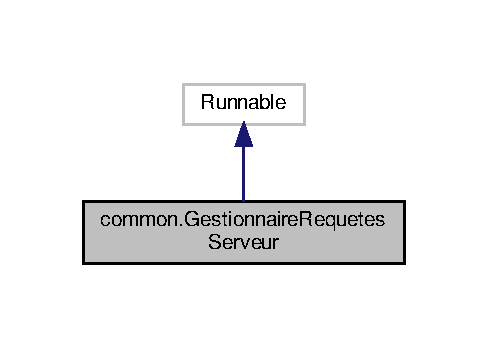
\includegraphics[width=234pt]{classcommon_1_1GestionnaireRequetesServeur__inherit__graph}
\end{center}
\end{figure}


Collaboration diagram for common.\+Gestionnaire\+Requetes\+Serveur\+:
\nopagebreak
\begin{figure}[H]
\begin{center}
\leavevmode
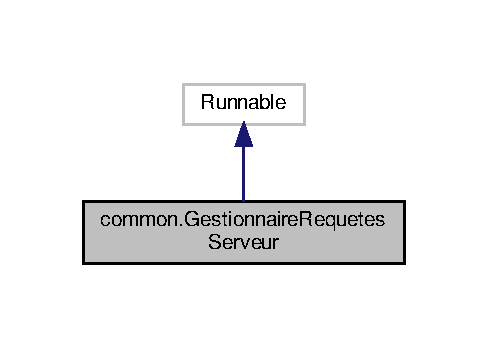
\includegraphics[width=234pt]{classcommon_1_1GestionnaireRequetesServeur__coll__graph}
\end{center}
\end{figure}
\subsection*{Public Member Functions}
\begin{DoxyCompactItemize}
\item 
\hyperlink{classcommon_1_1GestionnaireRequetesServeur_af17b749cf30080cec886973a7cc2f2aa}{Gestionnaire\+Requetes\+Serveur} (Socket soc\+Service, \hyperlink{classcommon_1_1GestionnaireFichier}{Gestionnaire\+Fichier} gestionnaire\+Fichier)  throws I\+O\+Exception 
\begin{DoxyCompactList}\small\item\em constructeur de \hyperlink{classcommon_1_1GestionnaireRequetesServeur}{Gestionnaire\+Requetes\+Serveur}. \end{DoxyCompactList}\item 
\mbox{\Hypertarget{classcommon_1_1GestionnaireRequetesServeur_a24848da2b934c89e632ac3c96df3bf8a}\label{classcommon_1_1GestionnaireRequetesServeur_a24848da2b934c89e632ac3c96df3bf8a}} 
void \hyperlink{classcommon_1_1GestionnaireRequetesServeur_a24848da2b934c89e632ac3c96df3bf8a}{run} ()
\begin{DoxyCompactList}\small\item\em methode pour lancer le traitement des requêtes d\textquotesingle{}un client \end{DoxyCompactList}\end{DoxyCompactItemize}


\subsection{Detailed Description}
Cette classe gere les requêtes d\textquotesingle{}un client. 

\subsection{Constructor \& Destructor Documentation}
\mbox{\Hypertarget{classcommon_1_1GestionnaireRequetesServeur_af17b749cf30080cec886973a7cc2f2aa}\label{classcommon_1_1GestionnaireRequetesServeur_af17b749cf30080cec886973a7cc2f2aa}} 
\index{common\+::\+Gestionnaire\+Requetes\+Serveur@{common\+::\+Gestionnaire\+Requetes\+Serveur}!Gestionnaire\+Requetes\+Serveur@{Gestionnaire\+Requetes\+Serveur}}
\index{Gestionnaire\+Requetes\+Serveur@{Gestionnaire\+Requetes\+Serveur}!common\+::\+Gestionnaire\+Requetes\+Serveur@{common\+::\+Gestionnaire\+Requetes\+Serveur}}
\subsubsection{\texorpdfstring{Gestionnaire\+Requetes\+Serveur()}{GestionnaireRequetesServeur()}}
{\footnotesize\ttfamily common.\+Gestionnaire\+Requetes\+Serveur.\+Gestionnaire\+Requetes\+Serveur (\begin{DoxyParamCaption}\item[{Socket}]{soc\+Service,  }\item[{\hyperlink{classcommon_1_1GestionnaireFichier}{Gestionnaire\+Fichier}}]{gestionnaire\+Fichier }\end{DoxyParamCaption}) throws I\+O\+Exception\hspace{0.3cm}{\ttfamily [inline]}}



constructeur de \hyperlink{classcommon_1_1GestionnaireRequetesServeur}{Gestionnaire\+Requetes\+Serveur}. 


\begin{DoxyParams}{Parameters}
{\em soc\+Service} & la socket de service qui permet de communiquer avec le client. \\
\hline
\end{DoxyParams}

\begin{DoxyExceptions}{Exceptions}
{\em I\+O\+Exception} & exception qui survient à la création du stream \\
\hline
\end{DoxyExceptions}


The documentation for this class was generated from the following file\+:\begin{DoxyCompactItemize}
\item 
Gestionnaire\+Requetes\+Serveur.\+java\end{DoxyCompactItemize}

\hypertarget{classclient_1_1mainClient}{}\section{client.\+main\+Client Class Reference}
\label{classclient_1_1mainClient}\index{client.\+main\+Client@{client.\+main\+Client}}
\subsection*{Static Public Member Functions}
\begin{DoxyCompactItemize}
\item 
\mbox{\Hypertarget{classclient_1_1mainClient_a0b28fb87463204b64524e5261b283d23}\label{classclient_1_1mainClient_a0b28fb87463204b64524e5261b283d23}} 
static void {\bfseries main} (String\mbox{[}$\,$\mbox{]} args)  throws Interrupted\+Exception 
\end{DoxyCompactItemize}


The documentation for this class was generated from the following file\+:\begin{DoxyCompactItemize}
\item 
main\+Client.\+java\end{DoxyCompactItemize}

\hypertarget{classserveur_1_1MainServeur}{}\section{serveur.\+Main\+Serveur Class Reference}
\label{classserveur_1_1MainServeur}\index{serveur.\+Main\+Serveur@{serveur.\+Main\+Serveur}}


Classe qui permet l\textquotesingle{}execution du serveur de transfert de fichiers.  


\subsection*{Static Public Member Functions}
\begin{DoxyCompactItemize}
\item 
\mbox{\Hypertarget{classserveur_1_1MainServeur_afe17c1452f1eaafbe93c797ff10bc824}\label{classserveur_1_1MainServeur_afe17c1452f1eaafbe93c797ff10bc824}} 
static void {\bfseries main} (String\mbox{[}$\,$\mbox{]} args)
\end{DoxyCompactItemize}


\subsection{Detailed Description}
Classe qui permet l\textquotesingle{}execution du serveur de transfert de fichiers. 

The documentation for this class was generated from the following file\+:\begin{DoxyCompactItemize}
\item 
Main\+Serveur.\+java\end{DoxyCompactItemize}

\hypertarget{classcommon_1_1Messages}{}\section{common.\+Messages Class Reference}
\label{classcommon_1_1Messages}\index{common.\+Messages@{common.\+Messages}}


cette classe gère les messages d\textquotesingle{}information et d\textquotesingle{}erreurs  


\subsection*{Public Member Functions}
\begin{DoxyCompactItemize}
\item 
void \hyperlink{classcommon_1_1Messages_a6069bc66b0eda8fdd5966a7c7a8a1a0a}{ecrire\+Message} (String message)
\begin{DoxyCompactList}\small\item\em écrit un message d\textquotesingle{}information. \end{DoxyCompactList}\item 
void \hyperlink{classcommon_1_1Messages_a5d8d6f3ce6024d78171f9e49de7f6136}{ecrire\+Erreur} (String message)
\begin{DoxyCompactList}\small\item\em écrit un message d\textquotesingle{}erreur. \end{DoxyCompactList}\end{DoxyCompactItemize}
\subsection*{Static Public Member Functions}
\begin{DoxyCompactItemize}
\item 
static \hyperlink{classcommon_1_1Messages}{Messages} \hyperlink{classcommon_1_1Messages_a96928a28b3f958fc717fca2c076f773c}{get\+Instance} ()
\begin{DoxyCompactList}\small\item\em singleton pour accéder à une instance unique de \hyperlink{classcommon_1_1Messages}{Messages} \end{DoxyCompactList}\end{DoxyCompactItemize}


\subsection{Detailed Description}
cette classe gère les messages d\textquotesingle{}information et d\textquotesingle{}erreurs 

\subsection{Member Function Documentation}
\mbox{\Hypertarget{classcommon_1_1Messages_a5d8d6f3ce6024d78171f9e49de7f6136}\label{classcommon_1_1Messages_a5d8d6f3ce6024d78171f9e49de7f6136}} 
\index{common\+::\+Messages@{common\+::\+Messages}!ecrire\+Erreur@{ecrire\+Erreur}}
\index{ecrire\+Erreur@{ecrire\+Erreur}!common\+::\+Messages@{common\+::\+Messages}}
\subsubsection{\texorpdfstring{ecrire\+Erreur()}{ecrireErreur()}}
{\footnotesize\ttfamily void common.\+Messages.\+ecrire\+Erreur (\begin{DoxyParamCaption}\item[{String}]{message }\end{DoxyParamCaption})\hspace{0.3cm}{\ttfamily [inline]}}



écrit un message d\textquotesingle{}erreur. 


\begin{DoxyParams}{Parameters}
{\em message} & message à écrire \\
\hline
\end{DoxyParams}
\mbox{\Hypertarget{classcommon_1_1Messages_a6069bc66b0eda8fdd5966a7c7a8a1a0a}\label{classcommon_1_1Messages_a6069bc66b0eda8fdd5966a7c7a8a1a0a}} 
\index{common\+::\+Messages@{common\+::\+Messages}!ecrire\+Message@{ecrire\+Message}}
\index{ecrire\+Message@{ecrire\+Message}!common\+::\+Messages@{common\+::\+Messages}}
\subsubsection{\texorpdfstring{ecrire\+Message()}{ecrireMessage()}}
{\footnotesize\ttfamily void common.\+Messages.\+ecrire\+Message (\begin{DoxyParamCaption}\item[{String}]{message }\end{DoxyParamCaption})\hspace{0.3cm}{\ttfamily [inline]}}



écrit un message d\textquotesingle{}information. 


\begin{DoxyParams}{Parameters}
{\em message} & message à écrire \\
\hline
\end{DoxyParams}
\mbox{\Hypertarget{classcommon_1_1Messages_a96928a28b3f958fc717fca2c076f773c}\label{classcommon_1_1Messages_a96928a28b3f958fc717fca2c076f773c}} 
\index{common\+::\+Messages@{common\+::\+Messages}!get\+Instance@{get\+Instance}}
\index{get\+Instance@{get\+Instance}!common\+::\+Messages@{common\+::\+Messages}}
\subsubsection{\texorpdfstring{get\+Instance()}{getInstance()}}
{\footnotesize\ttfamily static \hyperlink{classcommon_1_1Messages}{Messages} common.\+Messages.\+get\+Instance (\begin{DoxyParamCaption}{ }\end{DoxyParamCaption})\hspace{0.3cm}{\ttfamily [inline]}, {\ttfamily [static]}}



singleton pour accéder à une instance unique de \hyperlink{classcommon_1_1Messages}{Messages} 

\begin{DoxyReturn}{Returns}
retourne une instance unique de \hyperlink{classcommon_1_1Messages}{Messages} 
\end{DoxyReturn}


The documentation for this class was generated from the following file\+:\begin{DoxyCompactItemize}
\item 
Messages.\+java\end{DoxyCompactItemize}

\hypertarget{classrequete_1_1Requete}{}\section{requete.\+Requete Class Reference}
\label{classrequete_1_1Requete}\index{requete.\+Requete@{requete.\+Requete}}


classe abstraite définissant une requête d\textquotesingle{}un client au serveur.  




Inheritance diagram for requete.\+Requete\+:
\nopagebreak
\begin{figure}[H]
\begin{center}
\leavevmode
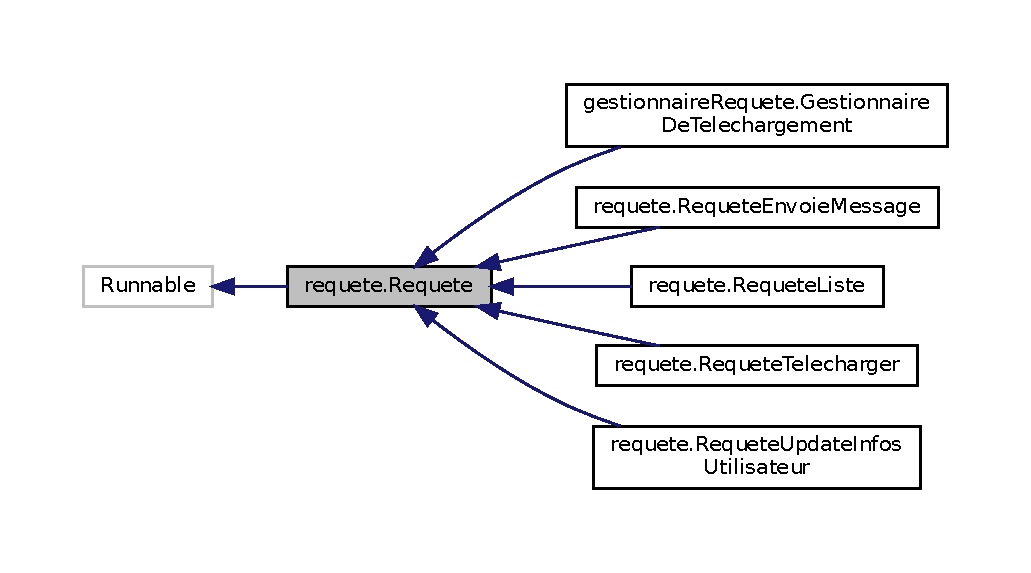
\includegraphics[width=350pt]{classrequete_1_1Requete__inherit__graph}
\end{center}
\end{figure}


Collaboration diagram for requete.\+Requete\+:
\nopagebreak
\begin{figure}[H]
\begin{center}
\leavevmode
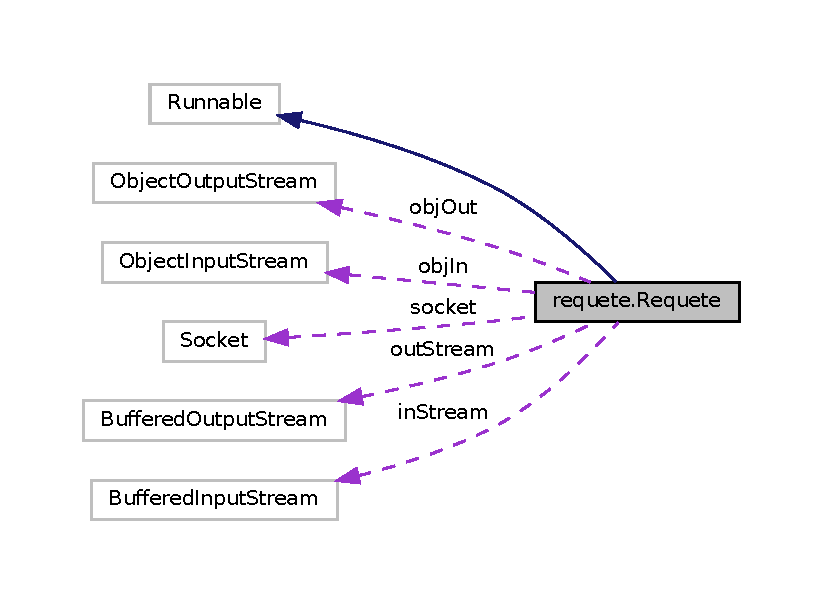
\includegraphics[width=350pt]{classrequete_1_1Requete__coll__graph}
\end{center}
\end{figure}
\subsection*{Public Member Functions}
\begin{DoxyCompactItemize}
\item 
\hyperlink{classrequete_1_1Requete_a6ed8eefb9335b37f2348f5c323a46b53}{Requete} (String adresse\+Serveur)
\begin{DoxyCompactList}\small\item\em constructeur de \hyperlink{classrequete_1_1Requete}{Requete}. \end{DoxyCompactList}\item 
\mbox{\Hypertarget{classrequete_1_1Requete_a919081397ea25302286d7077e3ece323}\label{classrequete_1_1Requete_a919081397ea25302286d7077e3ece323}} 
void \hyperlink{classrequete_1_1Requete_a919081397ea25302286d7077e3ece323}{run} ()
\begin{DoxyCompactList}\small\item\em methode pour lancer le thread. \end{DoxyCompactList}\end{DoxyCompactItemize}
\subsection*{Protected Member Functions}
\begin{DoxyCompactItemize}
\item 
void \hyperlink{classrequete_1_1Requete_a4adc60edaa26be2f8d9b4e4b0a1377cd}{envoyer\+Requete} (String requete)
\begin{DoxyCompactList}\small\item\em envoie une requête au serveur. \end{DoxyCompactList}\item 
\mbox{\Hypertarget{classrequete_1_1Requete_a139183d42763866d351b3569c858b169}\label{classrequete_1_1Requete_a139183d42763866d351b3569c858b169}} 
void \hyperlink{classrequete_1_1Requete_a139183d42763866d351b3569c858b169}{terminer} ()
\begin{DoxyCompactList}\small\item\em fermer les differents éléments du Thread. \end{DoxyCompactList}\end{DoxyCompactItemize}
\subsection*{Protected Attributes}
\begin{DoxyCompactItemize}
\item 
\mbox{\Hypertarget{classrequete_1_1Requete_ac459a04e0e05713cf40d2810141730f1}\label{classrequete_1_1Requete_ac459a04e0e05713cf40d2810141730f1}} 
String {\bfseries ip\+Serveur}
\item 
\mbox{\Hypertarget{classrequete_1_1Requete_a09be09377c9ce1174e027c9bc852c0ab}\label{classrequete_1_1Requete_a09be09377c9ce1174e027c9bc852c0ab}} 
int {\bfseries port\+Serveur}
\item 
\mbox{\Hypertarget{classrequete_1_1Requete_a487b0b95bcb22cd79e17b8ba2756daa6}\label{classrequete_1_1Requete_a487b0b95bcb22cd79e17b8ba2756daa6}} 
Buffered\+Input\+Stream {\bfseries in\+Stream}
\item 
\mbox{\Hypertarget{classrequete_1_1Requete_aec10f73f1c9edcba8a6aeffbd9dc932b}\label{classrequete_1_1Requete_aec10f73f1c9edcba8a6aeffbd9dc932b}} 
Buffered\+Output\+Stream {\bfseries out\+Stream}
\item 
\mbox{\Hypertarget{classrequete_1_1Requete_a8bbfc163d41bdf7d3ed614e0341a1bc8}\label{classrequete_1_1Requete_a8bbfc163d41bdf7d3ed614e0341a1bc8}} 
Socket {\bfseries socket}
\end{DoxyCompactItemize}


\subsection{Detailed Description}
classe abstraite définissant une requête d\textquotesingle{}un client au serveur. 

\subsection{Constructor \& Destructor Documentation}
\mbox{\Hypertarget{classrequete_1_1Requete_a6ed8eefb9335b37f2348f5c323a46b53}\label{classrequete_1_1Requete_a6ed8eefb9335b37f2348f5c323a46b53}} 
\index{requete\+::\+Requete@{requete\+::\+Requete}!Requete@{Requete}}
\index{Requete@{Requete}!requete\+::\+Requete@{requete\+::\+Requete}}
\subsubsection{\texorpdfstring{Requete()}{Requete()}}
{\footnotesize\ttfamily requete.\+Requete.\+Requete (\begin{DoxyParamCaption}\item[{String}]{adresse\+Serveur }\end{DoxyParamCaption})\hspace{0.3cm}{\ttfamily [inline]}}



constructeur de \hyperlink{classrequete_1_1Requete}{Requete}. 


\begin{DoxyParams}{Parameters}
{\em adresse\+Serveur} & adresse et port du serveur de la forme \char`\"{}\+I\+P\+:\+P\+O\+R\+T\char`\"{}. \\
\hline
\end{DoxyParams}


\subsection{Member Function Documentation}
\mbox{\Hypertarget{classrequete_1_1Requete_a4adc60edaa26be2f8d9b4e4b0a1377cd}\label{classrequete_1_1Requete_a4adc60edaa26be2f8d9b4e4b0a1377cd}} 
\index{requete\+::\+Requete@{requete\+::\+Requete}!envoyer\+Requete@{envoyer\+Requete}}
\index{envoyer\+Requete@{envoyer\+Requete}!requete\+::\+Requete@{requete\+::\+Requete}}
\subsubsection{\texorpdfstring{envoyer\+Requete()}{envoyerRequete()}}
{\footnotesize\ttfamily void requete.\+Requete.\+envoyer\+Requete (\begin{DoxyParamCaption}\item[{String}]{requete }\end{DoxyParamCaption})\hspace{0.3cm}{\ttfamily [inline]}, {\ttfamily [protected]}}



envoie une requête au serveur. 


\begin{DoxyParams}{Parameters}
{\em requete} & requete envoyé au serveur. \\
\hline
\end{DoxyParams}


The documentation for this class was generated from the following file\+:\begin{DoxyCompactItemize}
\item 
Requete.\+java\end{DoxyCompactItemize}

\hypertarget{classrequete_1_1RequeteListe}{}\section{requete.\+Requete\+Liste Class Reference}
\label{classrequete_1_1RequeteListe}\index{requete.\+Requete\+Liste@{requete.\+Requete\+Liste}}


Cette classe permet de créer un Thread qui va demander à un serveur la liste des fichiers qu\textquotesingle{}il contient.  




Inheritance diagram for requete.\+Requete\+Liste\+:
% FIG 0


Collaboration diagram for requete.\+Requete\+Liste\+:
% FIG 1
\subsection*{Public Member Functions}
\begin{DoxyCompactItemize}
\item 
\hyperlink{classrequete_1_1RequeteListe_abf11f2cbe8b9eb9eae7621dff966ebd5}{Requete\+Liste} (String adresse\+Serveur)
\begin{DoxyCompactList}\small\item\em constructeur de la classe \hyperlink{classrequete_1_1RequeteListe}{Requete\+Liste} \end{DoxyCompactList}\item 
\mbox{\Hypertarget{classrequete_1_1RequeteListe_a744397e5813266c362903f65965e0e4e}\label{classrequete_1_1RequeteListe_a744397e5813266c362903f65965e0e4e}} 
void \hyperlink{classrequete_1_1RequeteListe_a744397e5813266c362903f65965e0e4e}{run} ()
\begin{DoxyCompactList}\small\item\em methode pour lancer le Thread. \end{DoxyCompactList}\end{DoxyCompactItemize}
\subsection*{Additional Inherited Members}


\subsection{Detailed Description}
Cette classe permet de créer un Thread qui va demander à un serveur la liste des fichiers qu\textquotesingle{}il contient. 

\subsection{Constructor \& Destructor Documentation}
\mbox{\Hypertarget{classrequete_1_1RequeteListe_abf11f2cbe8b9eb9eae7621dff966ebd5}\label{classrequete_1_1RequeteListe_abf11f2cbe8b9eb9eae7621dff966ebd5}} 
\index{requete\+::\+Requete\+Liste@{requete\+::\+Requete\+Liste}!Requete\+Liste@{Requete\+Liste}}
\index{Requete\+Liste@{Requete\+Liste}!requete\+::\+Requete\+Liste@{requete\+::\+Requete\+Liste}}
\subsubsection{\texorpdfstring{Requete\+Liste()}{RequeteListe()}}
{\footnotesize\ttfamily requete.\+Requete\+Liste.\+Requete\+Liste (\begin{DoxyParamCaption}\item[{String}]{adresse\+Serveur }\end{DoxyParamCaption})\hspace{0.3cm}{\ttfamily [inline]}}



constructeur de la classe \hyperlink{classrequete_1_1RequeteListe}{Requete\+Liste} 


\begin{DoxyParams}{Parameters}
{\em adresse\+Serveur} & adresse et port du serveur de la forme \char`\"{}\+I\+P\+:\+P\+O\+R\+T\char`\"{}. \\
\hline
\end{DoxyParams}


The documentation for this class was generated from the following file\+:\begin{DoxyCompactItemize}
\item 
Requete\+Liste.\+java\end{DoxyCompactItemize}

\hypertarget{classrequete_1_1RequeteTelechargerBlocFichier}{}\section{requete.\+Requete\+Telecharger\+Bloc\+Fichier Class Reference}
\label{classrequete_1_1RequeteTelechargerBlocFichier}\index{requete.\+Requete\+Telecharger\+Bloc\+Fichier@{requete.\+Requete\+Telecharger\+Bloc\+Fichier}}


cette classe va télécharger un bloc de fichier depuis un serveur.  




Inheritance diagram for requete.\+Requete\+Telecharger\+Bloc\+Fichier\+:
\nopagebreak
\begin{figure}[H]
\begin{center}
\leavevmode
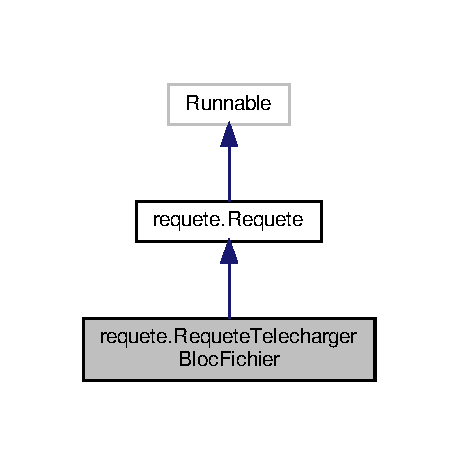
\includegraphics[width=220pt]{classrequete_1_1RequeteTelechargerBlocFichier__inherit__graph}
\end{center}
\end{figure}


Collaboration diagram for requete.\+Requete\+Telecharger\+Bloc\+Fichier\+:
\nopagebreak
\begin{figure}[H]
\begin{center}
\leavevmode
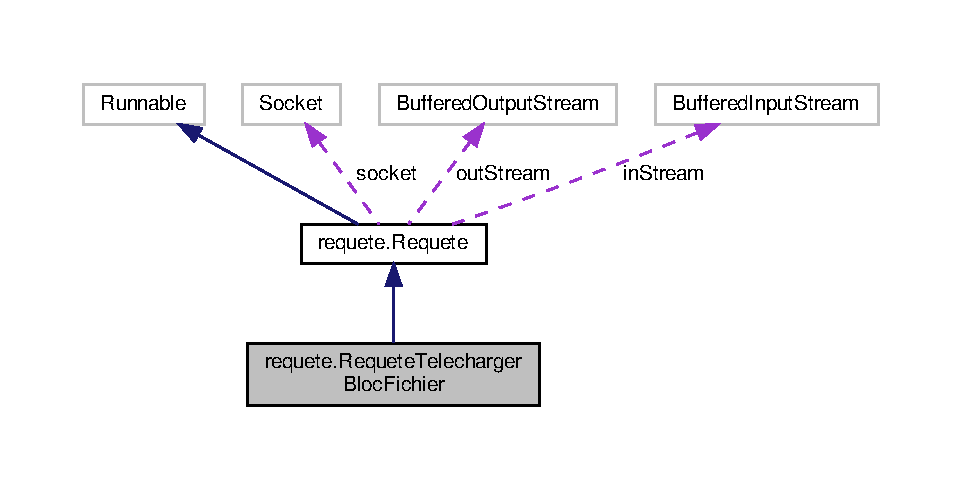
\includegraphics[width=350pt]{classrequete_1_1RequeteTelechargerBlocFichier__coll__graph}
\end{center}
\end{figure}
\subsection*{Public Member Functions}
\begin{DoxyCompactItemize}
\item 
\hyperlink{classrequete_1_1RequeteTelechargerBlocFichier_aff47f4619365925874158d0721f392e6}{Requete\+Telecharger\+Bloc\+Fichier} (String adresse\+Serveur, String nom\+Fichier, \hyperlink{classcommon_1_1GestionnaireFichier}{Gestionnaire\+Fichier} gestionnaire\+Fichier, String bloc\+Debut, String bloc\+Fin)
\begin{DoxyCompactList}\small\item\em télécharge une partie d\textquotesingle{}un fichier. \end{DoxyCompactList}\item 
\mbox{\Hypertarget{classrequete_1_1RequeteTelechargerBlocFichier_aca582462ab48dda6d3eaa26b6ca7b976}\label{classrequete_1_1RequeteTelechargerBlocFichier_aca582462ab48dda6d3eaa26b6ca7b976}} 
void \hyperlink{classrequete_1_1RequeteTelechargerBlocFichier_aca582462ab48dda6d3eaa26b6ca7b976}{run} ()
\begin{DoxyCompactList}\small\item\em methode pour lancer le Thread. \end{DoxyCompactList}\end{DoxyCompactItemize}
\subsection*{Additional Inherited Members}


\subsection{Detailed Description}
cette classe va télécharger un bloc de fichier depuis un serveur. 

\subsection{Constructor \& Destructor Documentation}
\mbox{\Hypertarget{classrequete_1_1RequeteTelechargerBlocFichier_aff47f4619365925874158d0721f392e6}\label{classrequete_1_1RequeteTelechargerBlocFichier_aff47f4619365925874158d0721f392e6}} 
\index{requete\+::\+Requete\+Telecharger\+Bloc\+Fichier@{requete\+::\+Requete\+Telecharger\+Bloc\+Fichier}!Requete\+Telecharger\+Bloc\+Fichier@{Requete\+Telecharger\+Bloc\+Fichier}}
\index{Requete\+Telecharger\+Bloc\+Fichier@{Requete\+Telecharger\+Bloc\+Fichier}!requete\+::\+Requete\+Telecharger\+Bloc\+Fichier@{requete\+::\+Requete\+Telecharger\+Bloc\+Fichier}}
\subsubsection{\texorpdfstring{Requete\+Telecharger\+Bloc\+Fichier()}{RequeteTelechargerBlocFichier()}}
{\footnotesize\ttfamily requete.\+Requete\+Telecharger\+Bloc\+Fichier.\+Requete\+Telecharger\+Bloc\+Fichier (\begin{DoxyParamCaption}\item[{String}]{adresse\+Serveur,  }\item[{String}]{nom\+Fichier,  }\item[{\hyperlink{classcommon_1_1GestionnaireFichier}{Gestionnaire\+Fichier}}]{gestionnaire\+Fichier,  }\item[{String}]{bloc\+Debut,  }\item[{String}]{bloc\+Fin }\end{DoxyParamCaption})\hspace{0.3cm}{\ttfamily [inline]}}



télécharge une partie d\textquotesingle{}un fichier. 


\begin{DoxyParams}{Parameters}
{\em adresse\+Serveur} & adresse du serveur et son port en format IP\+:P\+O\+RT. \\
\hline
{\em nom\+Fichier} & nom du fichier à télécharger. \\
\hline
{\em gestionnaire\+Fichier} & le gestionnaire de fichier. \\
\hline
{\em bloc\+Debut} & numéro du premier bloc à télécharger. \\
\hline
{\em bloc\+Fin} & numéro du dernier bloc à télécharger. \\
\hline
\end{DoxyParams}


The documentation for this class was generated from the following file\+:\begin{DoxyCompactItemize}
\item 
Requete\+Telecharger\+Bloc\+Fichier.\+java\end{DoxyCompactItemize}

\hypertarget{classrequete_1_1RequeteTelechargerFichier}{}\section{requete.\+Requete\+Telecharger\+Fichier Class Reference}
\label{classrequete_1_1RequeteTelechargerFichier}\index{requete.\+Requete\+Telecharger\+Fichier@{requete.\+Requete\+Telecharger\+Fichier}}


cette classe va télécharger un fichier depuis un serveur.  




Inheritance diagram for requete.\+Requete\+Telecharger\+Fichier\+:
% FIG 0


Collaboration diagram for requete.\+Requete\+Telecharger\+Fichier\+:
% FIG 1
\subsection*{Public Member Functions}
\begin{DoxyCompactItemize}
\item 
\hyperlink{classrequete_1_1RequeteTelechargerFichier_ad2f914dd2883d44935c00df622f8c60a}{Requete\+Telecharger\+Fichier} (String adresse\+Serveur, String nom\+Fichier, \hyperlink{classcommon_1_1GestionnaireFichier}{Gestionnaire\+Fichier} gestionnaire\+Fichier)
\begin{DoxyCompactList}\small\item\em télécharge un fichier depuis un serveur. \end{DoxyCompactList}\item 
\mbox{\Hypertarget{classrequete_1_1RequeteTelechargerFichier_a46bf87e436bf43a7695f7f7d264f5e2c}\label{classrequete_1_1RequeteTelechargerFichier_a46bf87e436bf43a7695f7f7d264f5e2c}} 
void \hyperlink{classrequete_1_1RequeteTelechargerFichier_a46bf87e436bf43a7695f7f7d264f5e2c}{run} ()
\begin{DoxyCompactList}\small\item\em methode pour lancer le Thread. \end{DoxyCompactList}\end{DoxyCompactItemize}
\subsection*{Additional Inherited Members}


\subsection{Detailed Description}
cette classe va télécharger un fichier depuis un serveur. 

\subsection{Constructor \& Destructor Documentation}
\mbox{\Hypertarget{classrequete_1_1RequeteTelechargerFichier_ad2f914dd2883d44935c00df622f8c60a}\label{classrequete_1_1RequeteTelechargerFichier_ad2f914dd2883d44935c00df622f8c60a}} 
\index{requete\+::\+Requete\+Telecharger\+Fichier@{requete\+::\+Requete\+Telecharger\+Fichier}!Requete\+Telecharger\+Fichier@{Requete\+Telecharger\+Fichier}}
\index{Requete\+Telecharger\+Fichier@{Requete\+Telecharger\+Fichier}!requete\+::\+Requete\+Telecharger\+Fichier@{requete\+::\+Requete\+Telecharger\+Fichier}}
\subsubsection{\texorpdfstring{Requete\+Telecharger\+Fichier()}{RequeteTelechargerFichier()}}
{\footnotesize\ttfamily requete.\+Requete\+Telecharger\+Fichier.\+Requete\+Telecharger\+Fichier (\begin{DoxyParamCaption}\item[{String}]{adresse\+Serveur,  }\item[{String}]{nom\+Fichier,  }\item[{\hyperlink{classcommon_1_1GestionnaireFichier}{Gestionnaire\+Fichier}}]{gestionnaire\+Fichier }\end{DoxyParamCaption})\hspace{0.3cm}{\ttfamily [inline]}}



télécharge un fichier depuis un serveur. 


\begin{DoxyParams}{Parameters}
{\em adresse\+Serveur} & adresse du serveur et son port en format IP\+:P\+O\+RT. \\
\hline
{\em nom\+Fichier} & nom du fichier à télécharger. \\
\hline
{\em gestionnaire\+Fichier} & le gestionnaire de fichier. \\
\hline
\end{DoxyParams}


The documentation for this class was generated from the following file\+:\begin{DoxyCompactItemize}
\item 
Requete\+Telecharger\+Fichier.\+java\end{DoxyCompactItemize}

\hypertarget{classcommon_1_1Serveur}{}\section{common.\+Serveur Class Reference}
\label{classcommon_1_1Serveur}\index{common.\+Serveur@{common.\+Serveur}}


Cette classe gère les fonctionnalitées de serveur.  




Inheritance diagram for common.\+Serveur\+:
\nopagebreak
\begin{figure}[H]
\begin{center}
\leavevmode
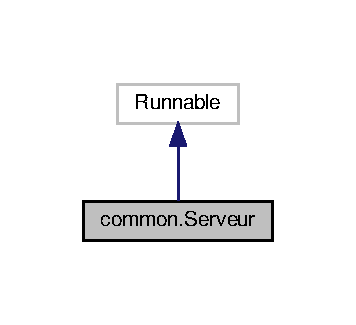
\includegraphics[width=171pt]{classcommon_1_1Serveur__inherit__graph}
\end{center}
\end{figure}


Collaboration diagram for common.\+Serveur\+:
\nopagebreak
\begin{figure}[H]
\begin{center}
\leavevmode
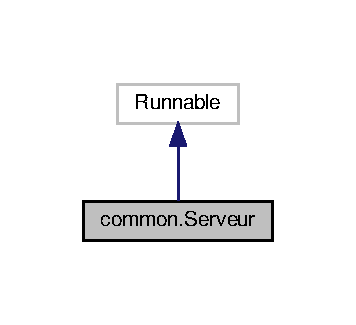
\includegraphics[width=171pt]{classcommon_1_1Serveur__coll__graph}
\end{center}
\end{figure}
\subsection*{Public Member Functions}
\begin{DoxyCompactItemize}
\item 
\hyperlink{classcommon_1_1Serveur_aef95775f670ec2ecd40e72111b125889}{Serveur} (int port, String adresse\+Dossier\+Partage)
\begin{DoxyCompactList}\small\item\em constructeur de la classe. \end{DoxyCompactList}\item 
void \hyperlink{classcommon_1_1Serveur_a14bedaf947acad1ebd395abf548b2a98}{run} ()
\begin{DoxyCompactList}\small\item\em Cette méthode permet de lancer le serveur. \end{DoxyCompactList}\end{DoxyCompactItemize}


\subsection{Detailed Description}
Cette classe gère les fonctionnalitées de serveur. 

\subsection{Constructor \& Destructor Documentation}
\mbox{\Hypertarget{classcommon_1_1Serveur_aef95775f670ec2ecd40e72111b125889}\label{classcommon_1_1Serveur_aef95775f670ec2ecd40e72111b125889}} 
\index{common\+::\+Serveur@{common\+::\+Serveur}!Serveur@{Serveur}}
\index{Serveur@{Serveur}!common\+::\+Serveur@{common\+::\+Serveur}}
\subsubsection{\texorpdfstring{Serveur()}{Serveur()}}
{\footnotesize\ttfamily common.\+Serveur.\+Serveur (\begin{DoxyParamCaption}\item[{int}]{port,  }\item[{String}]{adresse\+Dossier\+Partage }\end{DoxyParamCaption})\hspace{0.3cm}{\ttfamily [inline]}}



constructeur de la classe. 


\begin{DoxyParams}{Parameters}
{\em port} & port d\textquotesingle{}écoute du serveur. \\
\hline
{\em adresse\+Dossier\+Partage} & adresse du dossier qui contient les fichier partagés par le serveur. \\
\hline
\end{DoxyParams}


\subsection{Member Function Documentation}
\mbox{\Hypertarget{classcommon_1_1Serveur_a14bedaf947acad1ebd395abf548b2a98}\label{classcommon_1_1Serveur_a14bedaf947acad1ebd395abf548b2a98}} 
\index{common\+::\+Serveur@{common\+::\+Serveur}!run@{run}}
\index{run@{run}!common\+::\+Serveur@{common\+::\+Serveur}}
\subsubsection{\texorpdfstring{run()}{run()}}
{\footnotesize\ttfamily void common.\+Serveur.\+run (\begin{DoxyParamCaption}{ }\end{DoxyParamCaption})\hspace{0.3cm}{\ttfamily [inline]}}



Cette méthode permet de lancer le serveur. 

cette méthode lance le serveur en ouvrant la socket de rendez-\/vous, la méthode va par la suite attendre la venue d\textquotesingle{}un client puis transferer chaque connexion au gestionnaire de client pour qu\textquotesingle{}il traite les requête de chaque client dans un Thread unique. 

The documentation for this class was generated from the following file\+:\begin{DoxyCompactItemize}
\item 
Serveur.\+java\end{DoxyCompactItemize}

%--- End generated contents ---

% Index
\backmatter
\newpage
\phantomsection
\clearemptydoublepage
\addcontentsline{toc}{chapter}{Index}
\printindex

\end{document}
